
The Getting Started section explains how to register with Overleaf, create a new project based on the \texttt{refman} template, then use Overleaf's editor interface to configure the project.

\subsection{Register}
Web access to Overleaf will be required throughout this guide. Ensure you have an Overleaf account by registering at \url{https://www.overleaf.com/register}. 

\begin{minipage}{\linewidth}
\fbox{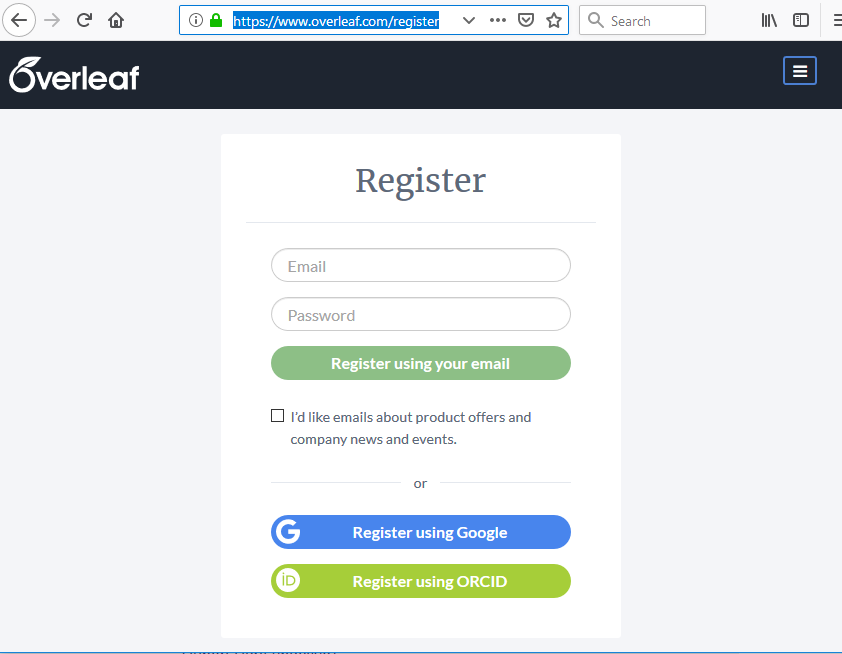
\includegraphics[width=\linewidth]{graphics/RegisterOverleaf.PNG}}
\captionof{figure}{Overleaf registration site \texttt{refman}}
\end{minipage}

Registering will give you access to Overleaf's powerful features including file management, cloud storage, and change tracking.

\subsection{New Project}
Navigate to
\url{https://www.overleaf.com/latex/templates/refman-format-technical-reference-manuals/jjrfdfpyxzvz} to start a new project with the \texttt{refman} template.

\begin{minipage}{\linewidth}
\centering
\fbox{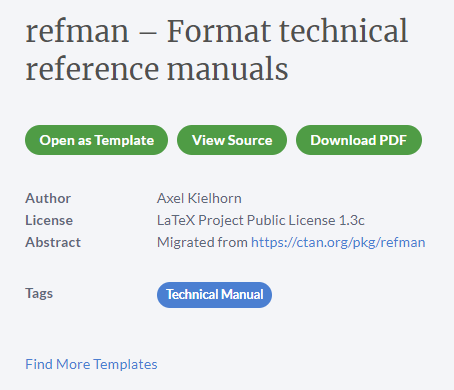
\includegraphics[width=.5\linewidth]{graphics/RefmanTemplate.PNG}}
\captionof{figure}{Overleaf registration site \texttt{refman}}
\end{minipage}

Click the 'Open as Template' button to create a new project based on the template; this will open the editor interface for the new project.

\begin{minipage}{\linewidth}
\fbox{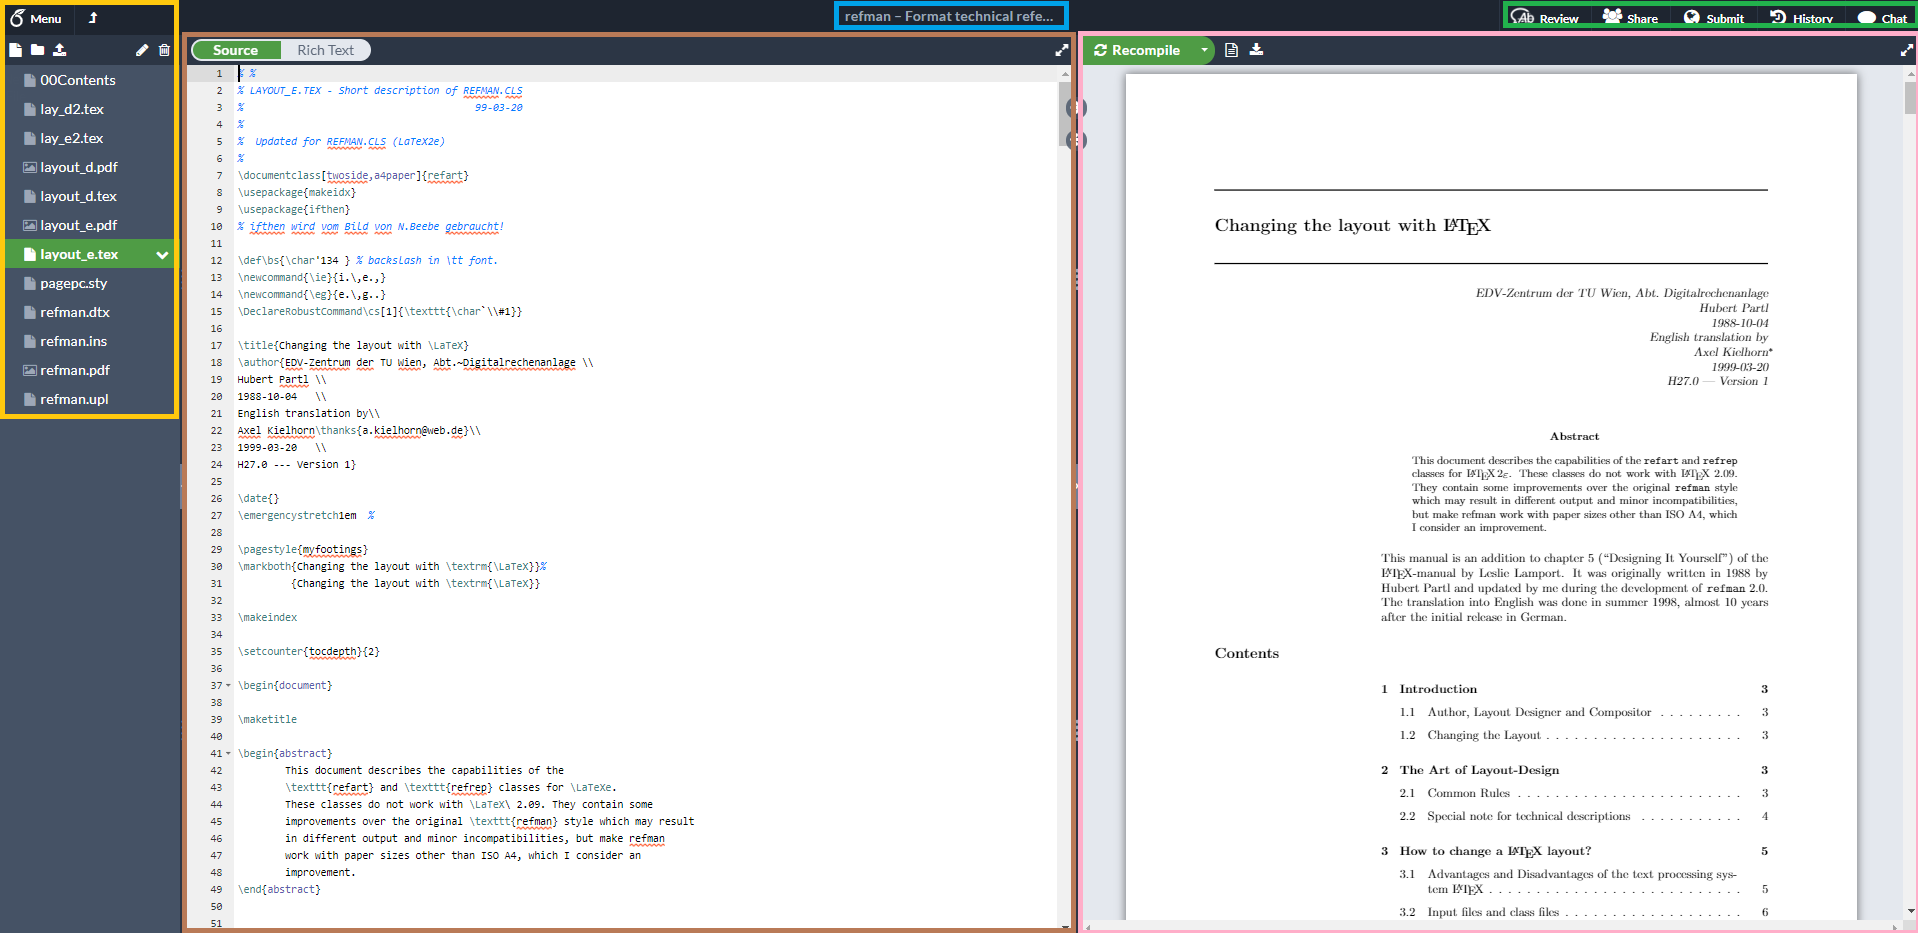
\includegraphics[width=\linewidth]{graphics/OverleafEditorInterface.PNG}}
\captionof{figure}{Overleaf Editor Interface}
\label{fig:EditorInterface}
\end{minipage}

The editor interface contains five interactable areas:
\begin{enumerate}
    \item \fcolorbox{black}{yellow}{Gold} left sidebar - File and project management
    \item \fcolorbox{black}{brown}{Brown} left textbox - \LaTeX\ document source editing
   \item \fcolorbox{black}{pink}{Pink} right textbox - Compiled \LaTeX\ document view
    \item \fcolorbox{black}{cyan}{blue} top-center title box - Modify title of Overleaf project
    \item \fcolorbox{black}{green}{Green} top-right button group - Change tracking and other collaboration tools
\end{enumerate}
See \url{https://www.overleaf.com/learn/latex/Tutorials} for comprehensive tutorials about the Overleaf web interface.

\subsection{Configuring Project}
The 'Title' and 'Main Document' of the project can now be configured.
\par
Highlight the top-center \textit{title box} to edit the project title (blue area in figure \ref{fig:EditorInterface}).

\begin{minipage}{\linewidth}
\fbox{
\includegraphics[width=\linewidth]{graphics/Rename.PNG}}
\captionof{figure}{Rename project title}
\end{minipage}

Locate and click the pencil symbol then enter your desired project name.

Now navigate to the left \textit{project management sidebar} (gold area in figure \ref{fig:EditorInterface}). Click the 'Menu' button in the top-left to open the \textit{project  settings window}.

\begin{minipage}{\linewidth}
\centering
\fbox{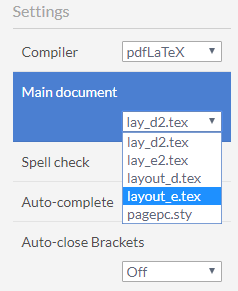
\includegraphics[width=.5\linewidth]{graphics/MainDocument.PNG}}
\captionof{figure}{Project Settings; Configuring main document}
\end{minipage}

Set the 'Main document' to the \path{layout_e.tex} document to compile \path{latex_e.tex} as the main document.
\par
The project is now configured and ready for adding content. See section \ref{sec:Basic Writing} to begin writing your \LaTeX\ project.